\title{CiALT abstract}
\documentclass[12pt]{article}
\usepackage[margin=1in]{geometry}
\usepackage{tikz} % for drawing figures
\usepackage{amsmath} % for equations
\usepackage{url} % for URLs
\usepackage{apacite}
\usepackage{graphicx}
\usepackage{float}
%\usepackage{parskip}
\usepackage{linguex} % ** special include in directory: for doing handy example labeling and bracketing
\usepackage[font=small]{caption}


\usepackage{times}

\newcommand{\sem}[1]{\mbox{$[\![$#1$]\!]$}}
\newcommand{\lam}{$\lambda$}
\newcommand{\gcs}[1]{\textcolor{blue}{[gcs: #1]}} 
\newcommand{\lsp}[1]{\textcolor{violet}{[lsp: #1]}} 
\newcommand{\lp}[1]{\textcolor{violet}{#1}}
\newcommand{\kj}[1]{\textcolor{green}{[kj: #1]}} 

\begin{document}

\begin{center}
\textbf{Child behavior in truth-value judgments: The pragmatics of ambiguity resolution}
\end{center}

Investigations of linguistic meaning rely crucially on truth-value judgments {({TVJs})}: whether a sentence can truthfully describe a given scenario. On the basis of such judgments, researchers have concluded that young children perform quite differently from adults when it comes to 
%understanding
{resolving}
ambiguous utterances with multiple potential meanings. For example, when adults hear ``Every horse didn't jump over the fence,'' they entertain two interpretations: either {\textit{none}} of the horses jumped or {\textit{not all}} of the horses jumped. {In contrast, five-year-olds}
%children 
usually only endorse the {\textit{none}} interpretation, rejecting the utterance in a {\textit{not-all}}
scenario where only two out of three horses jumped. However, subtle changes to the 
%truth-value judgment 
{TVJ} task setup make children{'s judgments} more adult-like. We summarize key results from the literature on child ambiguity resolution, noting three core variables {(two pragmatic, one processing)} that affect children's disambiguation behavior. We also highlight the {complex} nature of the 
%truth-value judgment 
{TVJ}
task children are being asked to engage in, which we then formally articulate using a cognitive computational model that specifies the role of each of these three variables in providing 
%truth-value judgments. 
{TVJs}.
The results suggest that pragmatic factors play a larger role than processing factors in explaining children's non-adult-like ambiguity resolution behavior, and the computational modeling framework allows us to understand why: by modeling the task itself, we see that the 
%truth-value judgment 
{TVJ}
data typically used to demonstrate children's difficulty with ambiguity {resolution} in fact require no disambiguation at all---just the ability to manage the pragmatics of the task. 

\textbf{Previous studies} suggest that children's scope resolution behavior is impacted by manipulations to the experimental context \cite{MuLid2006,viau2010priming,gualmini2008question,gualmini2008rise}. Specifically, experimenters have manipulated world knowledge about likely scenarios (e.g., how likely horses are to succeed), the Question-under-Discussion (QUD), and the priming of specific scope interpretations (i.e., surface vs.~inverse).  
{Two of these} variables concern children's ability to manage the pragmatic context: 
%\lsp{I reordered these to match the order you described them above}
modulating expectations about the world being described, and
understanding what the topic of conversation is.
{The other}
variable concerns children's processing ability: how easy it is to grammatically access the different interpretations. 
Importantly, it is not obvious from any of the existing experimental manipulations how to tease apart the independent contributions of these components. 

\textbf{We model} the pragmatics of ambiguity resolution within the Bayesian Rational Speech Act ({{RSA}}) framework \cite{GoodmanFrank2016} to capture and independently manipulate the contributions of each of these contextual and grammatical processing factors. The framework views language understanding as a social reasoning process. A listener interprets an utterance by reasoning about a cooperative speaker who is trying to inform a naive listener about the world. Our model is a ``lifted-variable'' variant wherein the ambiguous utterance's semantics gets parameterized by interpretation-fixing variables (i.e., the relative scope): Hearing an ambiguous utterance, a pragmatic listener reasons jointly about the true state of the world (i.e., how many horses succeeded), the likely QUD (i.e., topic of conversation), and the scope interpretation the speaker had in mind. The full lifted-variable RSA model appears in Fig.~1. Given that the available experimental data involve 
%truth-value judgments, 
{TVJs,}
we follow \citeA{degen2014lost} and \citeA{tessler2016manuscript} in modeling participants' behavior as a pragmatic speaker's (relative) endorsement of an utterance for an observed situation. Specifically, we model whether a speaker would endorse the ambiguous utterance as a description of the observed state, or prefer to say nothing at all. The pragmatic speaker makes this decision by reasoning about the probability that a pragmatic listener (who is reasoning about a speaker reasoning about a literal listener) would arrive at the correct state from the utterance. 

\textbf{Results} appear in Fig.~2, which plots the probability of a pragmatic speaker endorsing the ambiguous utterance (\textit{Every horse didn't succeed}) in a situation where two out of three horses succeeded. We see a stronger role for context management (as realized in priors on the world state and the QUD) than for grammatical processing (as realized in the prior on scope interpretations). Our model predicts the highest rates of utterance endorsement {will} occur when resolving the scope ambiguity is \emph{irrelevant} for communicating successfully about the {\textit{not-all}} world---that is, when expectations favor total success (i.e., $w$=3), or when the QUD asks if \emph{all?}~of the horses succeeded. In either case, both scope interpretations {(\textit{none} and \textit{not all})} serve to inform a listener, either that the \emph{a priori} likely $w$=3 does not hold, or that the answer to the \emph{all?}~QUD is \emph{no}.  These results suggest that the observed non-adult-like behavior (i.e., failure to endorse the utterance in a {\textit{not-all}} scenario) likely stems more from children's beliefs about the world of the experiment and about the topic of conversation, rather than any difficulty grammatically deriving the inverse scope interpretation. 


\begin{figure}[H]
  \begin{equation*}
  \begin{aligned}
P_{S_{2}} (u | w) &\propto \ exp(log \sum_{i,q} P_{L_{1}} (w, i, q | u))\\
 P_{L_{1}} (w, i, q | u) &\propto  \ P_{S_{1}} (u | w, i, q) \cdot P(w) \cdot P(i) \cdot P(q)\\
 P_{S_{1}} (u | w, i, q) &\propto  \ exp (\alpha \cdot log(L_{0}(x | u, i, q)))\\
  P_{L_{0}} (x | u, i, q) &\propto \ \sum_{w}\delta_{x=[\! [ q ]\! ](w)} \cdot P_{L_{0}} (w | u, i)\\
  P_{L_{0}} (w | u, i) &\propto \ \delta_{[\![u]\!]^{i}(w)} \cdot P(w)
  \end{aligned}
  \end{equation*}
  \vspace{-1em}
  \caption{Full RSA model: A pragmatic speaker ($S_2$) chooses an utterance $u$ to signal a state of the world $w$ to a pragmatic listener ($L_1$). Hearing an ambiguous utterance, $L_1$ reasons jointly about the true state of the world $w$ (0, 1, 2, or 3 horses succeeded), the likely QUD $q$ (\emph{did no horses succeed?}, \emph{did all horses succeed?}, \emph{how many horses succeeded?}), and the scope interpretation $i$ (surface vs.~inverse) that the speaker ($S_1$) had in mind. $S_1$ reasons about a naive listener ($L_0$), who reasons about which world $w$ is intended, given the semantics of utterance $u$ parameterized by the scope interpretation $i$ and the QUD $q$.}
  \end{figure}

\vspace{-1em}
\begin{figure}[H]
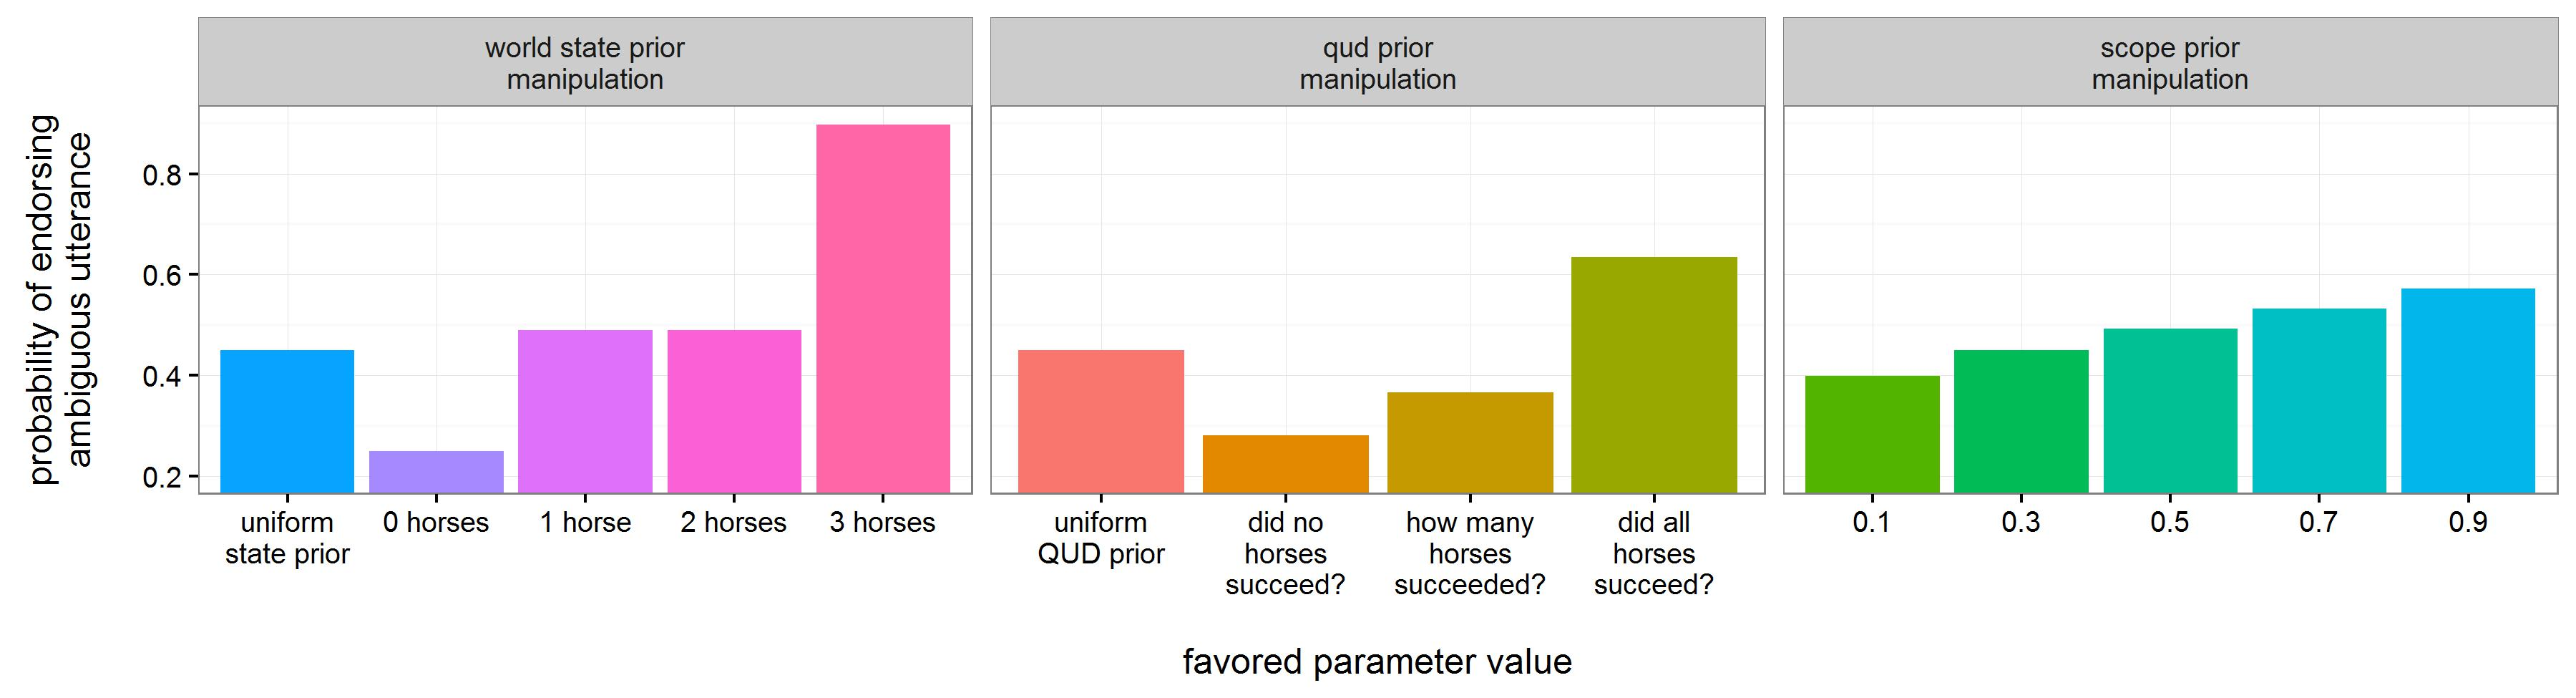
\includegraphics[width = \textwidth]{1.jpg}
\label{fig:graphs}
\vspace{-2em}
\caption{
%\lsp{Did you want to use the updated figure from KJ's advancement that manipulates the world prior as a horse success rate?}
Model predictions: Probability that a pragmatic speaker would endorse an ambiguous utterance (i.e., \emph{Every horse didn't succeed}) in a 
{\textit{not-all}}
scenario where two out of three horses did. Lower probability of endorsement corresponds to less adult-like (i.e., more child-like) behavior. For the contextual variables (world state, QUD), the favored world state or QUD is the one that has most of the prior probability weight ($P(favored) = 0.9$). For the grammatical processing variable (scope), the prior corresponds to how strongly the inverse scope is favored. }
\end{figure}

\bibliographystyle{apacite}
\setlength{\bibleftmargin}{.125in}
\setlength{\bibindent}{-\bibleftmargin}

\bibliography{bib}

\end{document}
